
\usepackage{ae}
\usepackage{array}
\usepackage{threeparttable}
\usepackage[T1]{fontenc}
\usepackage[utf8]{inputenc}
\usepackage{graphicx}
\usepackage{multicol}
\usepackage{rotating}
\usepackage{float}
\usepackage{listings}
\usepackage{lastpage}
\usepackage{dsfont}
\usepackage{amsmath, amssymb, amsfonts, amstext, xspace}
\usepackage{color}
\usepackage{transparent}
\usepackage{colortbl}
\usepackage{multirow}
\usepackage{caption}
\usepackage{epstopdf}
\usepackage{svg}
\usepackage{subfig}
\usepackage{fp}
\usepackage{mathtools}
\usepackage{longtable}
\usepackage[toc]{appendix}
\usepackage{tabularx}
\usepackage{anyfontsize}
\usepackage{pdfpages}
\usepackage{tikz}

\usepackage{pgfplots}
\pgfplotsset{compat=1.8}
\usepgfplotslibrary{statistics}
%\usepackage{minted}
\usepackage{subfig}
% adapt title and author
\usepackage{titling} % https://tex.stackexchange.com/questions/27710/how-can-i-use-author-date-and-title-after-maketitle

\usepackage[pdftitle={},pdfsubject={},pdfauthor={}]{hyperref}

% comment in this line if you are writing your bachelor thesis
\newcommand*{\BACHELOR}{}
% Adjust your information
\title{Chatbot-assisted Community Analysis}
\subtitle{\ifdefined\BACHELOR Bachelor \else Master \fi Thesis \ifdefined\PROPOSAL
		\PROPOSAL
	\fi}
\date{April 6, 2020}
\newcommand{\firstname}{Ben Aziz}
\newcommand{\lastname}{Lakhoune}
\newcommand{\matrNo}{380163}
\newcommand{\email}{ben.lakhoune@rwth-aachen.de}
\newcommand{\studyProgram}{\ifdefined\BACHELOR Bachelor \else Master \fi Computer Science}

% Adjust first supervisor information
\newcommand{\firstsupervisor}{PD Dr. Ralf Klamma}
\newcommand{\firstsupervisorchair}{Chair of Information Systems}
\newcommand{\firstsupervisoruniversity}{RWTH Aachen University}

% Adjust second supervisor information
\newcommand{\secondsupervisor}{Prof. Dr. Matthias Jarke}
\newcommand{\secondsupervisorchair}{Chair of Information Systems}
\newcommand{\secondsupervisoruniversity}{RWTH Aachen University}


% Adjust advisor information
\newcommand{\firstadvisor}{Alexander Neumann}
\newcommand{\firstadvisorchair}{Chair of Information Systems}
\newcommand{\firstadvisoruniversity}{RWTH Aachen University}

% comment these lines out if you have only one advisor
%\newcommand{\secondadvisor}{second advisor}
%\newcommand{\secondadvisorchair}{chair of second advisor}
%\newcommand{\secondadvisoruniversity}{RWTH Aachen University}


\addtolength{\evensidemargin}{-7mm}\addtolength{\oddsidemargin}{7mm}
\newcolumntype{M}[1]{>{\centering\arraybackslash}m{#1}}
\captionsetup[subfloat]{font=scriptsize, labelformat=parens, labelsep=space, listofformat=subparens}

\newcolumntype{L}[1]{>{\raggedright\let\newline\\\arraybackslash\hspace{0pt}}m{#1}}

\definecolor{grey}{rgb}{0.8,0.8,0.8}
\definecolor{red}{rgb}{1,0,0}
\definecolor{green}{rgb}{0,1,0}
\definecolor{yellow}{rgb}{1,1,0}
\definecolor{lightblue}{rgb}{0,0,0.5}
\definecolor{lightgray}{rgb}{.95,.95,.95}
\definecolor{darkgray}{rgb}{.4,.4,.4}
\definecolor{purple}{rgb}{0.65, 0.12, 0.82}

\newcommand{\blankpage}{
	\ifdefined\PROPOSAL
	\else
		\newpage
		\thispagestyle{empty}
		\mbox{}
		\newpage
	\fi
}

\graphicspath{{../../figures/}}


\title{Evaluation}

\begin{document}

\maketitle

\section*{Task 0 - Joining the Slack workspace}
    
     
\begin{itemize}
    \item Use the following link
    to join the Slack workspace if you are not a member yet
    \url{https://join.slack.com/t/mensacommunity/shared_invite/zt-nf09nfmb-EsChPf76BwKsUUlaRJqFqw}
    \begin{figure}[h]
        \centering
        
\includegraphics[height=7cm]{../presentation/frame.png}
    \end{figure}
    \item Use your email adress to sign in, or use Google Sign-in
    \begin{itemize}
    \item You might need to confirm your email adress
    \item Open your email account
    \item You should have received an email from Slack (Also check your spam folder)
    \item  Click the link inside the email. 
    \end{itemize}
    \item You should now be  in the Slack workspace
    \begin{itemize}
        \item If you have the Slack app you can click the popup \emph{Open in Slack}
        \item If you don't possess the Slack app you can also use it in the browser.
    \end{itemize}
    \item Locate the bot in the left taskbar near the bottom under Apps
\end{itemize}

\begin{figure}[h]
    \centering
    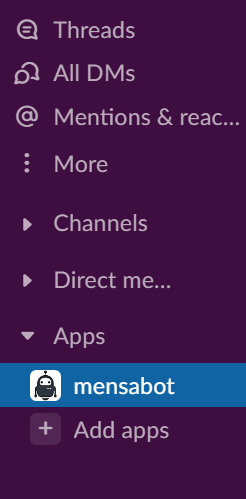
\includegraphics[height=7cm]{bot.png}
\end{figure}


      
\section*{Task 1 - Getting to know the bot}
\subsection*{Getting the menu}
\begin{itemize}
    \item Write a greeting message (e.g. Hello)
    \item You can type \textbf{help} to see a list of the capabilities of the bot
    \item Ask the bot to get the menu for your local mensa (canteen)
    \begin{itemize}
      \item Mensas might be closed
      \item Try using Aachen, Mensa Academica or Aachen, Mensa Vita
    \end{itemize}
    \item The bot might ask you, if you want to set a default city. Asnwer with an appropriate message
\end{itemize}
\subsection*{Making a review}
\begin{itemize}
    \item Ask the bot to make a review (e.g. I want to add a review)
    \item The review process should now be starting 
    \item The bot will ask you a series of questions
    \begin{itemize}
      \item Which mensa you went to and which meal you had (e.g. I went to Aachen, Mensa Academica and had the Klassiker) 
      \item Pay attention to write the category of the dish in the same manner that it is displayed on the menu
      \item How many stars out of 5 you would give your meal
      \item The bot will ask you to leave a comment
    \end{itemize}
\end{itemize}

\section*{Task 2 - Make a visualization}

\begin{itemize}
    \item Ask the bot to make a review Visualization
    \item The bot will ask for a measure. Ask the bot to list all measures
    \item Choose one of the measures 
    \item The bot will respond with the appropriate visualization
\end{itemize}


\section*{Task 3 - Update the success model}
\begin{itemize}
    \item Use the bot to get the success model
    \item Aks the bot to update the success model
    \item The bot will ask you to choose which success dimension you want to edit
    \item Choose a dimension by providing a number
    \item The bot will now ask you which success factor you want to edit
    \item Choose one by providing a number or add one by choosing an name for the factor
    \item Select one of the measures to add it to your factor. 
    \item The bot will now add the factor to the model.
    \item You can verify that it was added by typing "get the success model" into the chat
    \item You can also visualize your new measure in the same way as described in Task 2 on the previous slide
\end{itemize}

\section*{Feedback}
  
\begin{itemize}
  \item Please fill out the following survey: \url{https://docs.google.com/forms/d/e/1FAIpQLSfHn9kDKvCtccT3wqAOMIe-whJYlDP1l2pYTJinhNhZiNunTA/viewform?usp=sf_link}
\end{itemize}

\end{document}